\section{目的與規格對照}
Lab 11（PDF 第 44--51 頁）要求分析線路 RC、掃描驅動器尺寸、掃描線長及比較相鄰導線耦合。本次保留講義三組線路參數及各組 W/L 尺寸：45 個驅動尺寸變體、30 個線長變體、180 個耦合變體，共三個 netlist、255 個變體，全部完成。

講義原本將三組資料標成 0.35/0.25/0.18 $\mu$m 製程，電源分別為 3.3/2.5/1.8 V。本次沒有這三套對應 MOS 製程模型，因此以 A/B/C 標示 RC 與幾何情境，三者均使用同一份所提供模型及 1 V 電源。結果可比較線路與尺寸效應，不能宣稱重現三個 foundry 製程的絕對延遲。

\section{電路、參數與手算}
使用講義的三段 $\pi$ 模型：三個串聯電阻各為 $R/3$，兩端電容各為 $C/6$，中間兩個電容各為 $C/3$，總電阻與總電容皆保持原值。Inv1 為驅動器，Inv2 為接收反相器。$t_1$ 是輸入到驅動器輸出，$t_2$ 是到接收器輸入，$t_3$ 是到接收器輸出；前兩者反相，第三者同相。

對 10 mm 線路，講義表 11.1 的 R/C 及重新相乘的 RC 如下。A 組原表列 3.17 ns，與 $1.7\times2.11=3.587$ ns 不一致；本次保留 R、C 欄位並依實際乘積計算，沒有把該印刷數字當成量測結果。

\begin{center}\small
\begin{tabular}{lllll}
\toprule
Set & R (k$\Omega$) & C (pF) & RC (ns) & $W_p/W_n/L$ ($\mu$m) \\
\midrule
A & 1.70 & 2.11 & 3.587 & 2.7 / 0.9 / 0.35 \\
B & 2.38 & 2.39 & 5.688 & 1.8 / 0.6 / 0.25 \\
C & 3.39 & 2.46 & 8.339 & 1.5 / 0.5 / 0.18 \\
\bottomrule
\end{tabular}
\end{center}
驅動器寬度乘上 N=1--15，接收器維持單位尺寸；線長掃描固定 N=5，長度由 1 至 10 mm，每 1 mm 一點。線路 R、C 均隨長度成正比，因此線路內部 RC 項約隨長度平方成長。

耦合模型有左、中、右三條線，中線為被觀察者，每段同時保留對地電容與線間電容。表 11.4 的每微米參數為：
\begin{center}\small
\begin{tabular}{lllll}
\toprule
Set & R ($\Omega/\mu$m) & $C_c$ (fF/$\mu$m) & $C_g$ (fF/$\mu$m) & $C_s$ (fF/$\mu$m) \\
\midrule
A & .17 & .08 & .07 & .14 \\
B & .24 & .09 & .05 & .14 \\
C & .34 & .10 & .04 & .14 \\
\bottomrule
\end{tabular}
\end{center}
對每一組情境，掃描中線上升／下降、相鄰線 R/R、R/不變、R/F、不變/不變、不變/F、F/F 六組模式，線長為 2/4/6/8/10 mm，完整形成 $3\times2\times6\times5=180$ 個變體。不變的相鄰輸入固定於 0 V；R/F 指各線最前端輸入的上升／下降。
\section{模擬設定與量測定義}
本次使用獨立提供的 MOS 模型，電源為 1.0 V、溫度為 $27\,^{\circ}$C，並保留講義的電路拓樸及下列比較條件。1 V 是本次模擬設定，並非由公開模型文件確認的元件額定值；不能把講義舊製程的數值當成此次模型的驗收值。

模擬使用 HSPICE S-2021.09、RUNLVL=6。表格取自實際原生量測結果，圖形由實際列印數據重繪；每個變體都完整重設掃描參數及溫度，避免前一個變體的設定殘留。數值求解完成與量測成功，不等於已驗證製程可靠度。加密模型區塊的內部警告仍無法完整檢視。
一般線路測試以 100 ps 輸入斜坡、180 ns 暫態與 20 ps 列印間距，包含兩種極性。耦合測試在 20 ns 施加單次 100 ps 斜坡，模擬至 120 ns，使用輸入及接收器輸出 50\% 交越差作延遲。保持足夠觀察窗，避免把長線尚未到達的轉換誤判為失敗。

\section{驅動尺寸與線長結果}
加大驅動器能改善近端延遲，但遠端延遲逐漸受線路本身限制。

\begin{figure}[htbp]
\centering
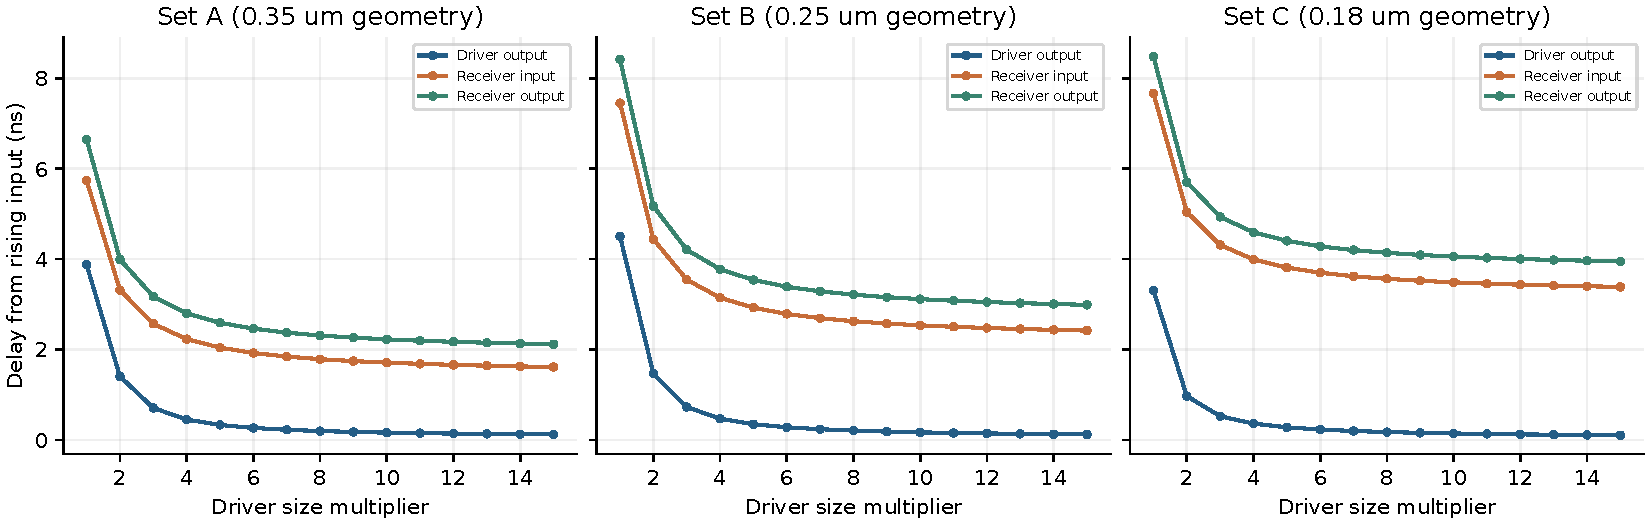
\includegraphics[width=\linewidth]{figures/wire_driver_sizing.pdf}
\caption{10 mm 線路的三個觀察點；曲線是輸入上升時的延遲。}
\end{figure}
\begin{figure}[htbp]
\centering
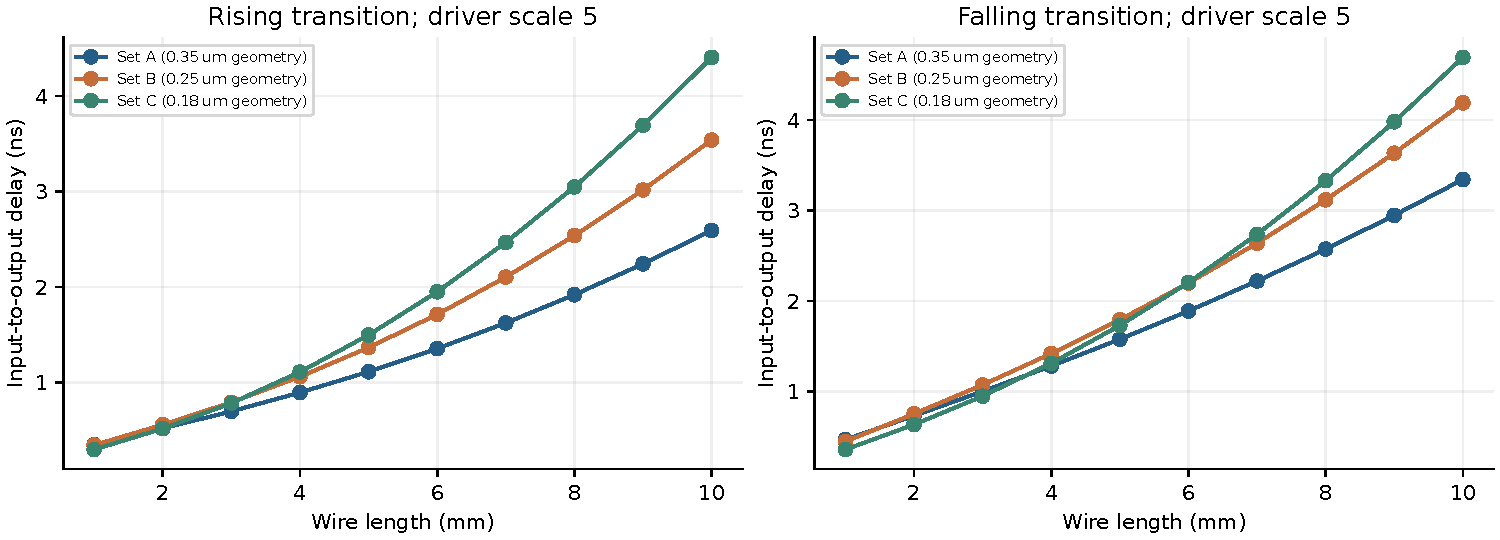
\includegraphics[width=\linewidth]{figures/wire_length.pdf}
\caption{固定 N=5 時，兩種極性的接收器輸出延遲隨線長增加。}
\end{figure}
\begin{center}\small
\begin{tabular}{llll}
\toprule
Set & N=1, $t_3$ (ns) & N=5, $t_3$ (ns) & N=15, $t_3$ (ns) \\
\midrule
A & 6.646 & 2.591 & 2.118 \\
B & 8.417 & 3.537 & 2.989 \\
C & 8.476 & 4.403 & 3.950 \\
\bottomrule
\end{tabular}
\end{center}
\section{耦合結果}
下表比較 10 mm 線路兩側同向與兩側反向切換的極端條件；所有數值取自本次實際模擬。

\begin{center}\small
\begin{tabular}{lllll}
\toprule
Set & Victim & Same (ns) & Opposite (ns) & Ratio \\
\midrule
A & R & 1.186 & 3.978 & 3.35 \\
A & F & 1.576 & 6.064 & 3.85 \\
B & R & 1.278 & 5.477 & 4.29 \\
B & F & 1.549 & 6.990 & 4.51 \\
C & R & 1.464 & 7.424 & 5.07 \\
C & F & 1.588 & 8.069 & 5.08 \\
\bottomrule
\end{tabular}
\end{center}
\begin{figure}[htbp]
\centering
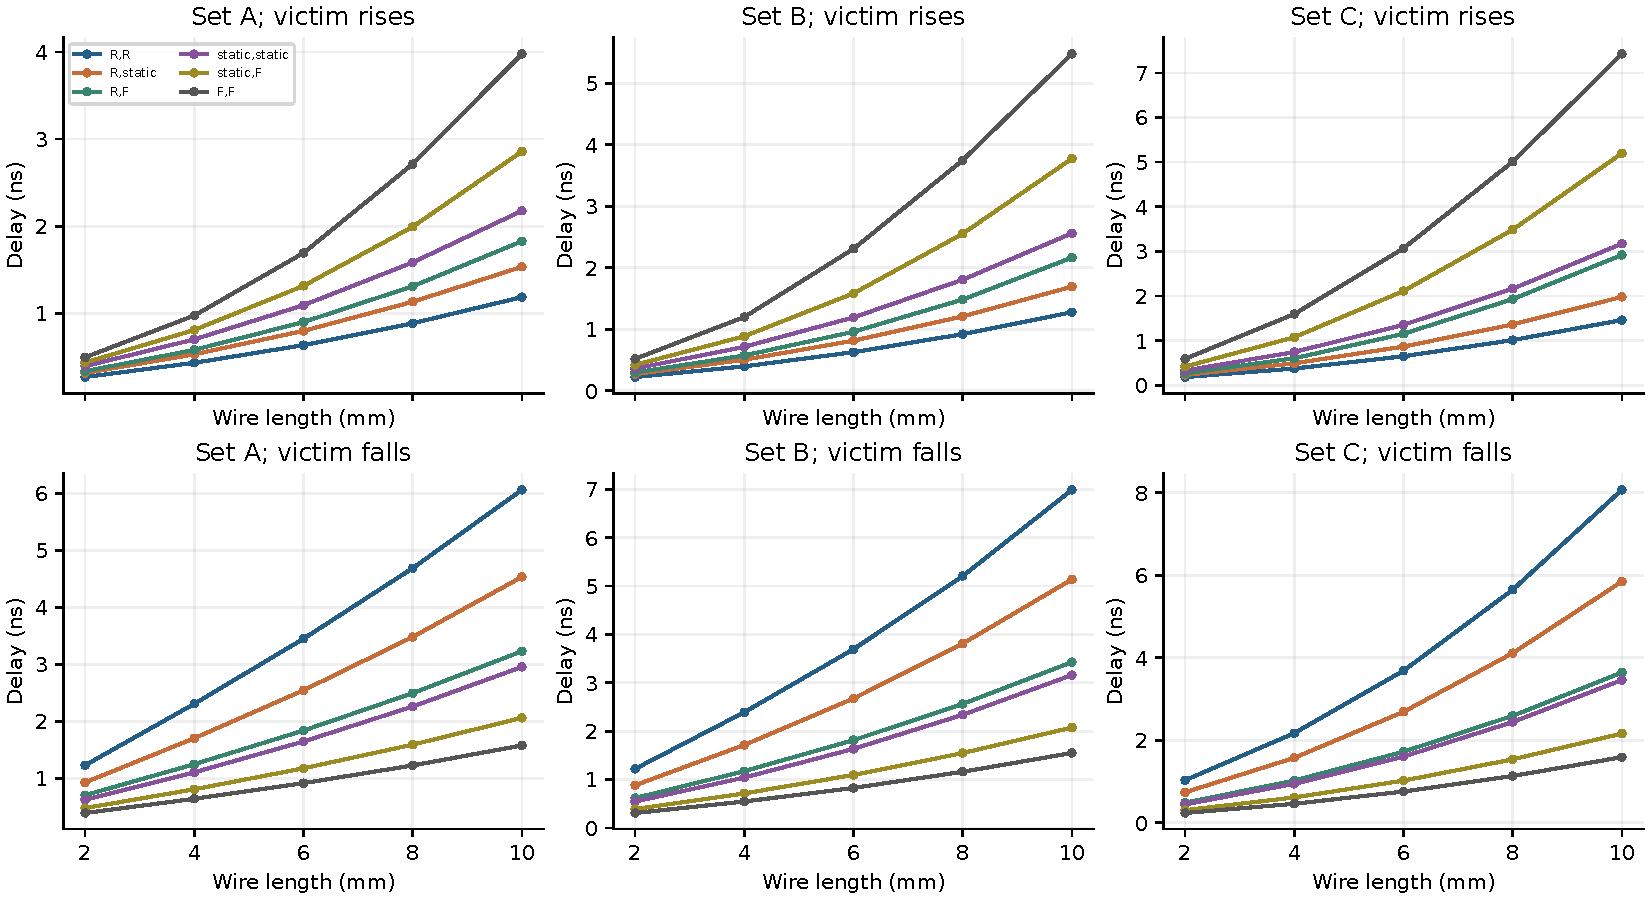
\includegraphics[width=\linewidth]{figures/wire_coupling.pdf}
\caption{完整六種相鄰輸入模式；R/F/不變的定義均在驅動器輸入端。}
\end{figure}
\section{討論與問題回答}
同向轉換時，兩端電位共同移動，線間電容上的電壓差較小；反向時差動擺幅變大，耦合負載增加。理想同步斜坡的近似式為 $C_{eff}=C_g+\sum C_c(1-dV_{adj}/dV_{victim})$：同向、相鄰不變、反向時，每條鄰線約分別貢獻 0、$C_c$、$2C_c$。實際線路的斜率及時間並不完全相同，因此延遲比例不會恰等於該電容量比例。

降低線路延遲可從較低電阻率金屬、加厚或加寬線路、降低介電常數、增加線距與縮短路徑著手；各方法會有面積、電容與佈線資源的取捨。電路面可分段插入適當尺寸的 repeater，或使用分級驅動；過度加大第一級只增加前級負擔，不能消除長線本身的 RC。屏蔽線可降低串擾，但會增加對地負載與金屬資源。

本次完成所有 RC 與耦合掃描條件；跨實際製程的絕對比較仍受限於缺少對應模型。本報告也沒有把講義表 11.5(c) 前幾個不連續數字當成驗證基準。

\section{可重現檔案}
本實驗上傳下列 netlist；模型設定以註解標記保留，模型檔與其路徑均不隨報告上傳。執行前須在本機補入合法可用的模型設定。
\begin{itemize}
\item \texttt{01\_driver\_sizing.sp}
\item \texttt{02\_wire\_length.sp}
\item \texttt{03\_coupled\_wires.sp}
\end{itemize}
每一個變體的完整量測值位於本 lab 的 \texttt{results}，並附代表性波形 CSV、分析結果與規格對照清單。波形 CSV 最多保留 2501 個均勻取樣點；直接量測未降採樣。完整原始 listing 留在本機。

